%!TEX root = pfe-book4.tex
%!TEX TS-program = pdflatex
%!TEX encoding = UTF-8 Unicode


\cleardoublepage
%\mainmatter
\chapter{Energy Around Us}
\label{ch-06}

\section{Sources of Energy}
In the final analysis, it will be seen that all the energy generated here on the earth comes from the sun. Tem­peratures of the order of millions of degrees rage in the deep interior of the sun. That is where reactions develop between atomic nuclei. They go by the name uncontrolled thermonuclear fusion.\footnote{The numbers in this section are a bit dated, especially in regard to energy production capacities. Solar power has made tremendous progress in the last decade or so. -- Damitr}

Man has harnessed these reactions and on the earth they release fabulous amounts of energy. The hydrogen bomb, for example. Research scientists are now attempt­ ing to bring the thermonuclear fusion reaction under control. That is the topic of this chapter.

Now that we have discussed the structure of nuclei we are ready to examine the sources of terrestrial energy. 

Under terrestrial conditions, we can obtain energy in three ways. First, we can extract energy from fuel (chem­ical or nuclear). This requires setting up a chain reac­tion in which molecules or atomic nuclei are combined or disrupted. Chemical fuels of practical value include coal, petroleum, and natural gas. Nuclear fuel for fission (breaking up of particles) includes uranium and thorium, and nuclear fuel for fusion (combining of particles) con­stitutes primarily the light element of hydrogen.

Second, the conversion of kinetic energy into work. Rivers can be made to generate electricity and thus ``work'' Hydraulic power (``white coal'') becomes one of the most important sources of energy. Here water falling from considerable heights generates electricity; this can be achieved by constructing dams or by utilizing natural waterfalls, like the Niagara Falls. Similarly, wind can be harnessed to convert energy into work turning the blades of a windmill. We shall see that wind (``blue coal'') must be taken seriously. Windmills are coming to life again on a much higher engineering level and will soon be making a substantial contribution to the energy bank. The same can be said of such an energy source as tidal waves.

The laws of thermodynamics suggest a third solution to the energy problem. In principle, it is always possible to design an engine that can use temperature differences. As we know, a transfer of heat from a hot body to a cool body can be partially converted into mechanical work. Now we encounter temperature differences in many places: in the earth's crust, in the oceans, and in the atmosphere. Going down into the interior of the earth (actually, of course, it amounts to digging slightly into the crust) we invariably observe an increase in temperature.

To repeat, all these three possibilities ultimately stem from the fact of solar radiation coming to the earth. The earth receives an insignificant portion of the energy radiated by solar rays. But even this minute bit is so colossal that for many years it will handle our needs and be enough to carry out the most fantastic projects.

But solar energy can also be utilized directly. The reader will recall that we have learned to convert radiant energy into electric current with the aid of photoelectric devices. As we know, the generation of electricity is the most important way of making energy serve practically.

Of course, in many cases both the internal energy of matter and the energy of the motion of water and wind can be utilized directly, bypassing the stage of conversion into electric current. However, perhaps in all cases, with the exception of aircraft and rockets, it is advisable to obtain electricity from the prime source at power plants and make the electric current serve our needs. The importance of electric energy will grow immeasurably as soon as we learn how to construct light-weight high-capacity storage batteries for electric automobiles in place of the heavy low-capacity ones now in use.

Before going on to a concrete discussion of energy sources, I wish to bring the attention of the reader once more to two important classifications of sources. First of all, there is an important dividing line between fuel and solar energy. In the former case, we are spending the wealth of the earth which cannot be replaced. Now the sun, the wind, and the water are sources for which we do not have to pay anything. They are free of charge in the sense that using their energies does not in any way diminish the wealth of the earth. Windmills do not reduce the amount of air in the atmosphere, the operation of hydropower plants does not take water out of the rivers, and solar-driven power-generating devices do not use up any terrestrial resources.

There is another classification. We have to protect nature at large -- the flora and fauna of the earth. This is a problem whose importance is hard to overestimate. Burning fuel is bad both because it depletes the material of the earth and also because it pollutes the ground, water, and air with enormous quantities of deleterious waste. Even hydroelectric power plants have their draw­ backs. Changes made in the water regimen of rivers can affect the climate and complicate the life cycles of the fish population of the world.

There can be no doubt that the optimal mode of obtaining energy is the direct utilization of the sun's radiation. 

Such are the principles. Now let us take up a more concrete discussion of the possibilities of energy utiliza­tion under terrestrial conditions and give some of the figures that can be found in the reference literature on power generation.

We start with solar energy. Every square metre on the outer boundary of the earth's atmosphere receives about \SI{1.4}{\kilo\watt} of energy (which is about 10 million kilocalories of energy in one year). Hundreds of kilograms of coal would be needed to generate that much heat. So how much heat does the earth as a whole receive from the sun?  Calculating the area of the earth and taking into account the nonuniform illumination of the earth's sur­face by the sun's rays, we obtain about \SI{d14}{\kilo\watt}. This is 100 000 times more energy than that produced by all the power sources on the earth: factories, power plants, automobile engines, aircraft engines; in other words, this is 100 000 times more power than the energy consumed by the entire population of the world (about a thousand million kilowatts).

Up to now, solar energy has hardly at all been touched. The point is this: although the overall figure is enormous, a good deal of the energy falls on the slopes of inacces­sible mountains, on the oceans that occupy most of the earth's surface, and on the sands of desert areas. What is more, only a relatively small amount of energy falls on any small area. Surely it would not be feasible to construct energy receivers over many square kilometres of surface. And, finally, solar energy can be converted into heat only in localities where there are regularly many sunny days during the year.

The thirst for power and tremendous advances in the production of semiconductor photoelectric cells have rad­ically changed the psychology of power engineers. There are many designs and even experimental units that focus solar radiation on thousands (in the future there will be millions, perhaps even thousands of millions) of photoelectric cells. And cloudy days and absorption of rays by the atmosphere are not serious deterrents. There can be no doubt that there is a great future in the direct utiliza­tion of solar energy.

Wind is now regarded in a different light too. Some twenty years ago wind was dismissed as a reasonable source of power. It has the same defect as solar energy, and that is that the amount of energy per unit area is relatively small. In order to generate power for factories, one would need windmills with vanes too large to be prac­ticable.

Another essential drawback is that the wind force is not a constant factor. All that relegates the energy of the wind, or ``blue coal'' as the poet says, to small engines (windmills). When the wind is up, these power plants generate electricity for agricultural machines and home lighting. If extra power is generated, it can be stored in storage batteries, which will take up the load in times of calm. Obviously, the windmill has only a sec­ondary role to play.

Today, engineers discussing the energy problem reason differently. Designs for electric power plants consisting of thousands of appropriately positioned ``windmills'' with enormous vanes are on the verge of being made into hardware. The use of wind will surely make an appre­ciable contribution to man's ever increasing needs.

Another gratuitous source of energy is moving water, the tidal waves of the ocean that constantly wash up onto the land, and the water of the rivers that flow to the seas and oceans. In 1969, hydroelectric power generation came to 115.2 thousand million kilowatt-hours in the USSR and 253.3 thousand million kilowatt-hours in the USA; however, utilization of water resources in the So­viet Union is only 10.5\% while in the United States it comes to 37\%.

These figures are impressive, but if we were deprived of all coal, petroleum, and other energy sources and only made use of hydro power -- even if all engineering opportunities were utilized for hydroelectric power generation -- we could not meet our requirements today.

What energy can be extracted from tidal waves? A great deal, although it is approximately one tenth the energy of rivers. Unfortunately, only a small portion of this energy can be harnessed. Because of the pulsating nature of the tides, there are many complications. However, Soviet and French engineers have found some practical ways of overcoming them. Today, tidal power stations ensure guaranteed outputs during hours of maximum consumption. In France, a tidal power station has been con­structed on the river Ranee, in the USSR there is a station at Kislaya Guba in the vicinity of Murmansk. This latter station is an experimental model for tidal power stations of 10 000 million watts (now in the design stage) to be built in bays of the White Sea.

Ocean water at considerable depths has temperatures \SI{10}{\celsius} to \SI{20}{\celsius} different from the surface layers. This offers possibilities of constructing a heat engine whose heater, in the medium latitudes, would be the upper layer of water and whose cooler would be the deep-lying layer. Such machines could have an efficiency of 1\% to 2\%. This of course is also a highly unconcentrated source of power.


\begin{figure}[!ht]
\centering

\includegraphics[width=\textwidth]{figures/fig-06-01.pdf}
\caption{Extracting the geothermal energy.}
\label{fig-6.1}
\end{figure}

Another gratuitous source of power is geothermal ener­gy (\figr{fig-6.1}). We will not discuss countries that have many geysers. There are not so many; and where there are, the heat of the geysers is utilized for industrial purposes. What we shouldn't forget is that two or three kilometres below any spot on the globe we encounter temperatures of the order of 150 to 200 degrees Celsius. The principle un­derlying a geothermal power station is obvious. Drill two channels. Cold water enters one and hot water comes out of the other.


\section{Fuel}
All the power sources described above have great ad­vantages over fuel. Fuel is burned. Utilizing the energy of coal, petroleum, and wood constitutes largely an irreplaceable destruction of terrestrial wealth.

What are the reserves of fuel here on earth? Ordinary fuel that burns when ignited with a match includes coal, petroleum, and natural gas. Their reserves are extremely limited. At the rate we are now using up petroleum, the known reserves will have been depleted completely by the beginning of the next century, the same goes for gas. There are somewhat larger reserves of coal, something like ten million million tons. The combustion of one kilogram of coal yields 7000 kilocalories of heat: (There are all kinds of fuel, and quality varies. This is naturally only a standard fuel used for measurement; it is a unit of comparison fuel used to compare different types of material.) Thus, the overall energy supplies of coal come to something on the order of \num{d20} kilocalories, which is roughly a thousand times the world's annual power consumption.

This thousand-year reserve is actually not much. A thousand years is a great deal if compared with the average human life span, but a person's life is only a moment when compared with the time of life on earth and with the existence of human civilization. What is more, power consumption is constantly increasing per head of the population. For this reason, if the fuel supplies consisted solely of petroleum and coal, the energy-reserve situation here on earth would have to be regarded as catastrophic.

But must we confine chemical fuel to the naturally found substances? Of course not. In a number of cases, it may prove that synthetic gaseous or liquid fuel is better than petroleum and natural gas.

In recent years much attention has been paid to the industrial production of hydrogen. As a fuel, hydrogen has many good points. It can be produced in limitless quantities in a variety of ways. It is readily available everywhere and so there are no transportation problems. Hydrogen can easily be purified of any undesirable impurities. In a number of cases it will be found that burning hydrogen directly for heat is the best thing. We can bypass the stage of converting it into elec­tricity.

At present, there are three main profitable ways of obtaining hydrogen: electrolytic, thermochemical de­composition, and, finally, irradiation of hydrogen--con­taining compounds with neutrons, ultraviolet rays, etc. It is even economically profitable to obtain hydrogen from coal and petroleum in nuclear reactors. In these cases, the hydrogen can be delivered by pipeline to the site of consumption, as is done with natural gas.

Concluding this brief survey of chemical fuels, let us now ask the question: What is the situation like concerning nuclear fuel? What are the reserves of nuclear fuel on the earth? Remember that only small amounts are consumed in nuclear reactors. One kilogram of nuclear fuel produces 2.5 million times more power than a kilo­gram of coal.

Approximate estimates show that the reserves of poten­tial nuclear fuel (why the word potential is used will be clear from what follows) come to about 2 million tons of uranium and 4 million tons of thorium. These are the fuels used to generate power in nuclear reactors based on the nuclear fission process. Will any other materials be added to these two elements? Perhaps. The number of nuclear reactions that produce energy is tremendous. The whole problem is how to make the process a chain reaction.

Let us first see what we are able to do at the present time. As follows from the preceding chapter, there is only one naturally found substance that can be used as nuclear fuel. That is the isotope uranium-235. The ura­nium mined in the earth contains 99.3\% of uranium-238 and only 0.7\% of uranium-235.

At first glance the simplest idea is this: isolate the necessary isotope, build reactors consisting of pieces (or rods) of that substance, introduce into the body of the reactor control rods that absorb neutrons and, thus, con­trol the nuclear reaction.

First of all, note that by absorbing neutrons and not allowing them to participate in the chain reaction we reduce the power of the reactor; in other words, we extract smaller amounts of energy per second from a unit mass of nuclear fuel. Now, if we slow down neutrons to thermal velocities and convert the ``fast'' neutrons generated in the disintegration of a nucleus into ``slow'' neutrons, that will be extremely useful in enhancing the efficiency of the reactor. This is because the nuclei of uranium-235 absorb slow neutrons with a far greater probability.

In all designs (except experimental reactors that haven't gone beyond the laboratory stage), the moderator has been either heavy water or ordinary water. Heavy water is good because it does not absorb neutrons at all, but it is not so good at slowing down neutrons as ordinary water is.

Thus, the best and simplest method is to isolate the uranium-235 isotope. That, as you recall, is a very expen­sive procedure. Chemical methods are useless: after all, these are chemically identical substances.

At present the most profitable method is by centrifug­ing. Before this operation can be started, we have to obtain a gaseous compound of uranium. The only such compound that is in the gaseous state at ordinary temper­atures is uranium hexafluoride. The mass difference of the gas molecules containing the isotopes uranium-238 and uranium-235 is so slight that the best centrifuge enriches the gas with lighter molecules only up to 12\%. In order to obtain uranium with 3\% of uranium-235 (such fuel can then be used in a nuclear reactor), the process has to be repeated 13 times. Clearly, the true solution of the engineering problem cannot be the obtaining of pure uranium-235.

But there is another and perhaps more important rea­son. Without uranium-235 it is impossible to convert the basic mass of uranium (and also thorium) into nuclear fuel. That is precisely why we spoke of potential fuel. As for the isotope uranium-235 itself, that fuel should hold off the onset of an energy famine for a hundred years or so. Therefore, if we want to utilize nuclear fuel for many long centuries, the approach must be quite differ­ent.

Nuclear fuel can be produced in the reactor itself, it turns out. We can first of all make plutonium-239, which is obtained from uranium-238, and, secondly, ura­nium-233, which is obtained from thorium-232. But there is no way of starting without uranium-235.

Reactors that generate energy and at the same time create new fuel are called breeders. It is possible to achieve a situation where the reactor will produce more new fuel than it consumes, that is, the reproduction factor is greater than unity.

To summarize then: technologically feasible ways of utilizing all the supplies of uranium and thorium are available. Consequently, by the most conservative esti­mates, there is enough fuel to last thousands of years.

And yet adding uranium and thorium to the fuel list does not fundamentally solve the energy problem for mankind; after all, there is a limit to the reserves of mineral wealth in the earth.

Now thermonuclear reactions are quite a different prop­osition. If we are able to tame the fusion of light nuclei, achieve a controlled self-sustaining thermonuclear reaction, then we can truly say that the energy problem has been resolved. How realistic is such a solution? Just recent­ly, physicists have obtained hydrogen plasma with temper­atures of about 60 million degrees. That is the temperature at which a thermonuclear reaction can take place. But the problem is to make such a reaction self-sustaining and to design a fusion (or thermonuclear) reactor. That is what we have yet to do.

There is so much thermonuclear energy in the waters of the oceans that it could satisfy all the power require­ments of humanity for a time span exceeding the age of the solar system -- a limitless source of energy, indeed.

We thus conclude our talk on fuel. Now let us examine the machines that make the fuel work.

\section{Electric Power Plants}

Of course, there are many instances of the direct util­ization of energy not in any way connected with the generation of electricity. Gas burning in the kitchen, the launching of a space vehicle (here, the recoil of the products of combustion sends the rocket into space), and even the old steam engines that are occasionally still found. In a number of cases, wind is converted directly into motion and energy.

But in most cases we need electric current -- to provide lighting, to power electric engines, to provide for electric traction, to ensure the operation of electric-welding and heating furnaces, to charge storage batteries, and to do many other things. At any rate, today we cannot con­ceive of delivering energy over distances in any way other than by electric current. It is therefore no exaggeration to say that the principal hero of technology remains the electric power plant.

There are still two basic industrial methods of turning the rotating parts of electric engines, the machines that generate electricity. If this work is done by the energy of falling water, we speak of \emph{hydroelectric power plants}; if the moving force is the pressure of steam on the blades of turbines, we speak of \emph{thermal power plants}.

Included in the class of thermal plants are \emph{atomic power plants}, although they actually differ from ordinary thermal plants in only one way: they use a different type of fuel. But in both cases we obtain heat that is used to produce steam.

The urbanite today is acquainted with the term central heating and power plant. These plants combine a supply of electricity with steam and hot water.

The energy of falling water has been utilized for cen­turies. The water wheel of the ancient mill is the proto­type of the modern hydraulic turbine. A stream of water hits the blades of the wheel and transfers part of its kinetic energy. The blade moves and rotates the wheel.

It is not so easy to position the blades of a wheel in order to obtain the best efficiency. This engineering problem is resolved by specialists in different ways, depending on how the water falls. Naturally, the greater the height (sometimes even 300 metres has been attained) from which the water falls the better the turbine performs.

The latest word in hydraulic-turbine construction are turbines exceeding \SI{500 000}{\kilo\watt} capacity. Since pow­er outputs of this kind are generated at rather low ro­tation speeds (of the order of 100 a minute), the new hydraulic turbines are colossal both in size and weight.

Depending on the direction of flow in the rotor, hy­draulic turbines are divided into axial-flow turbines and radial-axial turbines. The Soviet Union has hydroturbines of the radial-axial class with power outputs of \SI{508}{\mega­\watt} and 7.5-metre rotors.

Hydroelectric power plants generate the cheapest elec­tricity, but they are several times more expensive to con­struct than thermal power plants and the construction period is much longer. In hydraulic power plants, hydro­turbines set in motion hydrogenerators. These are very large synchronous machines mostly with vertical shafts. In such a machine, the diameter of the rotor is 7 to 10 times its length and in some of the largest machines it exceeds 15 metres. This is necessary for the machine to operate stably for variable speeds of the hydroturbine that rotates it. The rotor of a hydrogenerator has a large number of salient poles. For example, the generators of the Dnieper hydropower station have 72 poles. A special direct-current generator (called an exciter) is used to feed the windings of the poles. Hydrogenerators operate at rather low speeds -- from 80 to 250 revolutions per minute.

The hydrogenerator of the Krasnoyarsk power station (\SI{500}{\mega­\watt}) operates at 93.8 revolutions per minute, has a 16-metre-diameter rotor and weighs 1640 tons. A 650-megawatt generator is being designed for the Sayano-Shushensky hydropower station.

As I have already pointed out, hydropower generation affects the environment in certain adverse ways. But nevertheless there can be no doubt that hydropower plants have definite advantages over thermal power plants. First of all, hydropower plants do not use up fuel, and we know that fuel is in short supply. Thermal power plants have yet another very great drawback. A considerable portion of the power generated in converting the energy of the fuel into electricity is unavoidably lost.

Still and all, something like four fifths of all the elec­tric power is generated at thermal power plants by means of turbogenerators in which the driving force is the pres­sure of steam.

To increase the efficiency of the generator, it is nec­essary to raise the temperature of the steam. This can obviously be attained only by simultaneously increasing the pressure. In modern thermal electric power plants with capacities ranging from 200 to \SI{300}{\mega­\watt}, the turbines operate at steam parameters of \SI{565}{\celsius} and 24 meganewtons per square metre.

But why are high temperatures needed? To put it sim­ply, a steam turbine utilizes the same phenomenon that makes the cover of the tea kettle jump up when the water begins to boil. In other words, in a steam turbine we see thermal energy transformed into mechanical energy, and then from mechanical energy to electricity. Now, in the first transformation (this can be proved rigorously), energy is lost to the extent of a portion equal to the ratio of the ambient temperature to the temperature of the steam.

It is definitely too bad that we have to go through the ``thermal stage'' in modern devices in order to extract energy. This transition always involves a very great loss of power, and the ideal power plant of the future is one in which energy of any origin can be converted directly into electricity. Since that most important problem is not yet solved, there is only one thing left; and that is to strive for the highest possible temperatures of steam, gas, or plasma.

Difficult as that is, we are still able to achieve efficiencies of about 40\% in thermal electric power plants. The steam power generator is an electric machine with a horizontal shaft. The rotor is manufactured together with the ends of the shaft as a single piece of forging made out of special turbo-rotor steel. This is done because the mechanical stresses due to the high speeds of 3000 revolutions per minute reach the very limits of modern materials. For that same reason, the rotor does not have any salient poles. Parts of its cylindrical surface have slots into which the field (excitation) winding is laid. A three-phase alternating-current winding is laid in the slots of the stator.

Because of enormous mechanical stresses, the diameter of the rotor is restricted, and so to obtain sufficient power the machine has to be stretched out in length.

The first Soviet \SI{500}{\kilo\watt} turbogenerators were man­ufactured at the Leningrad ``Elektrosila'' plant in 1925. In 1964, the ``Elektrosila'' works turned out a turbogen­erator exactly 1000 times more powerful than the first one -- \SI{500000}{\kilo\watt}.

The desire to obtain more power from a single machine without increasing the already enormous dimensions has led to very complicated designs. For instance, to reduce losses in the windings of the stator, they are made in the form of hollow copper conductors in which water constant­ly flows. The excitation winding is cooled with hydrogen under a pressure of about 4 atmospheres. The use of hydrogen, which is 14 times less than the density of air, made it possible to increase the power of the turbogen­erators by 15\% to 20\%.

The five-year plan of 1976-1980 calls for the manufac­ture of turbogenerators of between 1000 and 1200 thousand kilowatts for thermal and atomic power plants.

One of the most interesting power plants in the world has been built in the Soviet Union. It is called U-25 and feeds about \SI{7000}{\kilo\watt} of electricity into the electric network. This is the world's largest plant for generating electricity by the method of \emph{magnetohydrodynamics}, MHD for short. An MHD-generator has no rotating parts.

The idea behind the operation of this interesting gen­erator is extremely simple. A flux of ions having con­siderable kinetic energy (this is, a jet of plasma) passes through a magnetic field across the magnetic lines of force. The ions are acted upon by the Lorentz force. Recall that the intensity of an induced electric field is propor­tional to the rate of ion flux and to the magnitude of magnetic induction. The electromotive force is perpen­dicular to the motion of the ions. That is the direction in which the current arises and closes on an external load. The electrodes that receive the current are in direct contact with the plasma.

Electric energy is generated due to the fall in energy of the plasma jet. An MHD-generator permits raising the efficiency of the power plant to 60\% and more.

The critical factor in generating cheap power from MHD is the magnetic field in the channel. This must be an intense field. An ordinary electromagnet with a copper coil can produce such a field but the magnet is then un­wieldy, complex in design, and expensive. What is more, it consumes a good deal of power itself. In this connection, designers have developed a new concept in designing magnets with a superconducting winding. This kind of magnet can generate the necessary magnetic field of re­quired intensity and with low power consumption and insignificant heating. Calculations have shown that the considerable expenses needed to obtain temperatures close to absolute zero justify themselves.

From this brief summary we see that traditional ways of increasing power generation have not yet exhausted themselves. However, one can hardly expect progress only along that road.

Aside from the fact that fuel supplies and opportunities for utilizing hydraulic sources of energy are coming to an end, one should not lose sight of the appreciable effect on the environment of the construction of new electric power plants. Ecologists have warned of the necessity of a very cautious approach to interfering in the life of rivers. Power engineers are reminded of the enormous quantities of ash that are thrown into the atmosphere in the course of fuel combustion. In one year, the earth's atmosphere receives 150 million tons of ash and about 100 million tons of sulphur. Particularly disquieting is the increase in the atmosphere of carbon dioxide. Every year, 20 thousand million tons of it are added to the atmosphere. During the past 100 years, the quantity of carbon dioxide in the atmosphere has increased 14\%.

There are two reasons for this growth: the destruction of vegetation on the earth and, what is most important, the release into the atmosphere of this ``gaseous ash'' in the combustion of ordinary fuel. This ceaseless increase can lead to ruinous consequences, of which the worst is an increase in the temperature of the atmosphere by 1.5 to 3 degrees. This might seem to be a small rise but in turn it can lead to an irreversible melting of the polar ice caps. Climatologists claim that the ultimate permissi­ble increase in carbon dioxide in the earth's atmosphere cannot exceed several tens percent.

\section{Nuclear Reactors}

As has already been pointed out, atomic power plants belong to the class of thermal electric power plants. The difference lies in the production of steam that is then directed onto the blades of a turbine. A nuclear reactor could be called a nuclear boiler because of the similarity of power generation.

A nuclear reactor is ordinarily in the form of a cylin­drical building. The walls have to be very thick and made of materials that absorb neutrons and gamma radia­tion. Reactors generating something like 1000 megawatts of electricity come in a variety of sizes depending on the fuel used, the method of moderating neutrons, and the mode of heat removal. But in all cases the size is impres­sive: the height of a 5- to 10-storey building and some ten or so metres in diameter.

Nuclear power engineering began to develop right after the Second World War. In the Soviet Union, the most important nuclear investigations were headed by Igor V. Kurchatov, a marvelous scientist and an excellent organizer.

In the Soviet Union and in other countries, a number of designs were tested. The first stumbling block is to decide the isotopic composition of the uranium or other nuclear fuel used. The engineer is then confronted with the form in which the fuel is supplied as a solution of uranium salts or in solid chunks. Solid fuel elements can come in a variety of shapes. Bars can be used but long rods appear to be most suitable. A very essential role is played by the geometry of the fuel elements (the positions they are placed in). Engineering calculations are needed to find the most suitable positions of the con­trol rods that absorb neutrons. Their movements (all auto­matic, naturally) must ensure the required value of the neutron multiplication factor.

Differences in the behaviour of slow (thermal) neu­trons and fast neutrons permit dividing reactors into two categories, namely, reactors with a neutron modera­tor and breeder reactors.

A reactor designed to operate on the principle of neu­tron moderation can use natural uranium. The amount of moderator has to be such as to prohibit large numbers of neutrons from being absorbed by uranium-238 nuclei. Now there are approximately 140 times more of these nuclei than there are uranium-235 nuclei. If there is not enough moderator, the neutrons will not diminish their speeds to the thermal level and will be absorbed by ura­nium-238 nuclei, and the chain reaction will come to a halt. A reactor operating on natural uranium or uranium slightly enriched in uranium-235 will still create a new fuel, plutonium. But much less plutonium will be pro­duced than the uranium nuclei that are ``burned'' up.

\newpage
\begin{center}

\includegraphics[width=0.8\textwidth]{figures/kurchatov.pdf}
\end{center}
{\small \textsf{{Igor Vasilievich Kurchatov [1902-1960]}} -- \textsf{\footnotesize prominent Soviet phys­icist and a remarkable organizer. He headed the work of the atom­ic project in the Soviet Union. He began his scientific career in the field of solid state physics and set up the theory of seignette-electrics (also known as ferroelectrics). At the beginning of the 1930s he began research in the physics of the atomic nucleus. Under his guidance, important studies were carried out in the field of nuclear isometry, the resonance absorption of neutrons, and arti­ficial radioactivity.}}

Up until just recently, most atomic power plants used thermal-neutron reactors. There are four types of such reactors: water-water reactors with ordinary water as the moderator and heat-transfer agent (coolant); graphite-water reactors with water coolant and graphite moderator; reactors in which heavy water is the moderator and ordinary water is the coolant; and, finally, graphite-gas-cooled reactors.

The reason why specialists in the field of atomic power engineering concentrated their attention on reactors oper­ating with thermal neutrons is apparently due to the fact that it is extremely difficult to enrich uranium in the 235 isotope. The reader will recall the remark made earlier that when only the isotope uranium-235 is used, enormous reserves of potential nuclear fuel are left untouched.

At the present time there is a tendency to have nuclear reactors operate on highly enriched fuel with no neutron moderator.

Suppose the mixture in the reactor consists of one part of uranium-235 and one part of uranium-238. In that case, the number of neutrons that fall out of the chain reaction due to capture by uranium-238 may exceed the number of neutrons fissioning nuclei of uranium-235 and sustaining the chain reaction. Such a reactor is termed a breeder. Depending on the geometry of the rods or bricks of nuclear active and potential fuel, it is possible to design breeder reactors with a great variety of percentage ratios of the two types of fuel and with different reproduction factors. Two examples will suffice to give the reader some idea of the parameters of nuclear reactors.
\begin{figure}[!ht]
\centering

\includegraphics[width=0.8\textwidth]{figures/fig-06-02.pdf}
\caption{A nuclear reactor design used in submarines.}
\label{fig-6.2}
\end{figure}


\figr{fig-6.2} is a general view of the design of a nuclear reactor used in submarines of the United States. The coolant here is ordinary water. Since ordinary water captures neutrons roughly 600 times more effectively than heavy water, such a reactor can operate only on uranium-238 enriched in uranium-235. Instead of the natural portion of 0.72\% in the fuel of these reactors we find from one to four percent of uranium-235. The reactor is capable of generating 1100 megawatts of electricity, is about 5 metres in diameter, has a height of 15 metres (a 5-sto­rey building) and wall thickness of about 30 centimetres. If such a reactor is charged with 80 tons of uranium oxide containing 3.2\% of uranium-235, it will operate 10 to 12 months (and then the rods have to be replaced). The water in the reactor heats up to \SI{320}{\celsius} and circulates under a pressure of about 300 atmospheres. The hot water turns to steam and is delivered to the blades of a tur­bine.

We now give a brief description of the design of a powerful breeder reactor to be built in France. It is called Superph\'enix.

The fuel will be a mixture of plutonium-239 and ura­nium-238. No moderator will be needed and so the neu­trons do not lose speed from the time of generation during nuclear fission up to an encounter with another atomic nuclei of the fuel.

The fact that the reactor employs fast neutrons makes for a high degree of compactness. The core of the reactor will not exceed 10 cubic metres. Thus, there will be a large liberation of heat per unit volume.

Heat removal cannot be done with water because water moderates neutrons. Liquid sodium will be used. Sodium melts at \SI{98}{\celsius} and boils at \SI{882}{\celsius} at atmospheric pressure. For technical reasons, the temperature of liquid sodium must not exceed \SI{550}{\celsius}. There is therefore no need to raise the pressure of the coolant (this is resorted to when the coolant is water).

The Superph\'enix reactor will have the following dimen­sions: inner diameter 64 metres, height about 80 metres. This is a big 20-storey building! The core of the reactor is in the form of a hexagonal prism made up (like a bundle of pencils) of thin rods each 5.4 metres in length. The fuel rods alternate with control rods.

There is no need (nor space) here to describe how the core of the reactor is cooled. Suffice it to say that it is done in three stages. A first loop contains sodium; it removes the heat from the reactor and delivers it to the boiler, where it is taken up by a second sodium loop. In the second heat exchanger, the heat is taken up by a third loop with a circulating water-steam mixture. Then follows the ordinary route to the steam turbine.

Calculations show that this setup should generate 3000 megawatts of thermal capacity and 1240 of electric­ity.

I cannot help stressing once again that the necessity of converting nuclear energy into electric energy passes through the thermal stage, leaving a poignant feeling of disappointment. It is something like installing an auto­mobile engine on a cart. But so far no one has come up with a better idea of how to bypass that stage, which creates perhaps the greatest difficulties in the construction of atomic power plants. Besides the common drawback of all thermal power plants, we have here the added necessity of including intermediate pipelines. This is done because we have to eliminate the unacceptable radioac­tivity of the water vapour entering the turbine.

Here are some more figures of this design. The maximum neutron flux per square centimetre per second is equal to \num{6.2d15}. The reproduction factor will be equal to 1.24. Used up fuel elements will be replaced once a year. In the first loop, there will be a flow of liquid sodium (technically called the mass flow rate) of 16.4 tons a second. Superheated steam will emerge under a pressure of 180 bars and at a temperature of \SI{490}{\celsius}.

A few words are in order about the ``ashes'' of nuclear fuel. A great number of radioactive isotopes appear in the fission of fuel nuclei. This is an uncontrollable process, but we have the opportunity of obtaining any isotopes we want merely by placing substances in the reactor. Such substances absorb neutrons and create new atoms.

Of course, radioisotopes can be obtained in accelerators by subjecting various materials to bombardment with protons or the nuclei of other elements.

The number of artificial elements obtained to date is very great. The ``empty'' places in the periodic table of elements have been filled up: elements No. 61, 85, and 87 do not have long-lived stable isotopes, and so there are none in nature. The Mendeleev table of elements has been extended. Elements above 92 are termed transura­nium elements. Each of the transuranium elements, all the way up to element 105, has been obtained in several isotopic variants.

Also, in addition to new chemical elements, large num­bers of radioisotopes have been obtained of those chemical elements that are encountered in the earth's crust in their stable form.

Radioisotopes have been widely used for many years in the sterilization of food products by gamma rays, in flaw detection, and as generators of electric power that use electrons produced in decay processes. This list could be extended considerably.

The usefulness of radioactive isotopes is, unfortunately, commensurate with the trouble engineers have in pro­tecting persons that deal with radioactive radiation.

Nuclear fuel waste contains 450 kinds of atoms, includ­ing uranium-237 and neptunium-239, which convert into neptunium-237 and plutonium-239.

Unlike coal or petroleum, nuclear fuel does not burn up completely. In a number of cases, nuclear reactors op­erate with enriched fuel containing between 2.5\% and 3.5\% of uranium-235. At some point, a reactor ceases to deliver energy because in the fission process a large num­ber of isotopes are produced that capture neutrons and prevent the fission process from developing. When a reactor is shut down, there is roughly 1\% of uranium-235 and a somewhat smaller amount of plutonium-239 left.

There can be no question of throwing away such ash containing large quantities of useful fuel. A big chemical works could be linked up with an atomic power plant. It would have to be completely automated since it would be handling highly radioactive materials. Special mea­sures would also have to be taken to protect personnel from gamma radiation.

At these plants, used fuel elements would be ground up and dissolved. The pure fuel (uranium and plutonium) could be extracted and returned for the manufacture of fresh fuel elements.

There still remains appreciable quantities of radioactive waste in the form of ``hot'' (radioactive) solutions that have to be buried. And what has to be ensured is that for many centuries the disposal sites will not be touched in any way.

Specialists are more or less optimistic. It is believed that the storing of cans (drums or barrels) of radioactive solutions up to one kilometre underground in specially selected spots should guarantee one hundred percent safe­ty. What kind of sites are suitable? That is a matter for geologists to decide. Only places safe from earthquakes, of course. Also, one must be sure there are no subter­ranean rivers or streams. Salt deposits have been found to satisfy such conditions. And, of course, the barrels cannot simply be dropped into a kilometre-deep well. To ensure dissipation of heat that the barrels would be emitting constantly, they will have to be dispersed at distances of at least up to 10 metres apart.

\section{Thermonuclear Energy}
We have already mentioned that chemical and nuclear reactions have much in common. Since heat is generated not only in reactions of decomposition but also, frequent­ly, in the combining of two molecules into one, we can expect that atomic nuclei behave in a similar manner.

It is not difficult to see what fusion reactions (com­bining of nuclei) would be advantageous from the energy point of view if we know the masses of the atomic nuclei.
The deuterium nucleus has a mass of 2.0146 mass units. If two nuclei fuse into one, we get \ce{^{4}He}, which has a mass of 4.0038 instead of $2 \times 2.0146 = 4.0292$. The excess mass of 0.0254 is equivalent to roughly \SI{25}{\mega\electronvolt} of energy, or \SI{4d-11}{\joule}. One gram of deuterium contains \num{0.3d24} atoms. Now if such a reaction took place, then two grams would yield \num{d13} joules of energy! It turns that the most promising are the fusion reactions of the heavy isotopes of hydrogen: deuterium, tritium. Even ordinary hydrogen can be put to use as thermonuclear fuel.

It is thus clear that atomic energy can be generated in two forms: the splitting up of heavy atomic nuclei in so-called fission reactions and the combining of light atomic nuclei in so-called fusion reactions, which are also called thermonuclear reactions.

Fusion reactions, if harnessed, could ensure our power needs for millions of years to come (and the level of the world's oceans would not go down perceptibly in the process of using the water). It would indeed be a limitless ocean of power, and at very low costs -- practically free of charge.

However, it is no easy job to harness this ``free'' source of power. The point is that all atomic nuclei are posi­tively charged. That means an enormous amount of energy is required to bring the nuclei close together.

The only way to obtain this energy is to convert a substance into the plasma state, which means stripping atomic nuclei of their clouds of electrons and then rais­ing the temperature of the plasma to a point where the nuclei begin to collide (collisions occur at distances of \num{d-13} centimetre apart) despite the electric repulsive forces.

Calculations turn out to be quite disappointing. The reader can himself try to calculate the amount of energy of electrostatic repulsion using the formula $e^{2}/r$ and then check the needed temperatures (you will have to recall the formula that relates the temperature and the kinetic energy of any particle). The answer is in the tens of millions of degrees.

To summarize, then, we need to produce a high-tem­perature plasma. There are two ways to do this: one has been in use for over two decades, the other is fifteen years or so younger.

The former method consists in creating a thermonu­clear reactor by ``driving'' the plasma into a magnetic bottle (that's what it's called).

If a magnetic field is imposed on a gas-discharge tube and is made to coincide in direction with the electric field, a plasma column is generated. We know that the charged particles of the plasma will describe helical tra­jectories. We can say that the particles move in a single ring surface current. The stronger the magnetic field the smaller the radius of the plasma column. The force acting on the current of charged particles via the magnetic field is what produces the column, which does not come in contact with the walls of the gas-discharge tube.

In principle, we have thus produced plasma that actu­ally ``hangs in the air''.

Calculations show that if the initial hydrogen pressure is of the order of 0.1 millimetre of mercury, the radius of the column is 10 centimetres, and the intensity of the discharge current is 500 000 amperes, then the temperature of the plasma should be sufficient for a fusion reac­tion to start up.

However, there are very many obstacles still in the way of a controlled thermonuclear (fusion) reaction. The plasma column is the main stumbling block. For a num­ber of reasons it is highly unstable and disintegrates almost instantaneously. The problem gets under control only if one is able to make a magnetic bottle with what might be called ``feedback'': that is, such that the random fluctuations that disrupt the column give rise to counteracting forces capable of restoring the column.

In the middle of 1978, a group of American physicists working at Princeton University succeeded in heating plasma to 60 million degrees. This success was achieved by using magnetic bottles called Tokamak (we discussed them in book three of this series). Tokamak -- a Soviet device -- is an acronym that stands for toroidal, chamber, magnet. The temperature attained is sufficient for the fusion of nuclei of deuterium and tritium. Since then, Soviet and also American scientists have attained still higher temperatures and better parameters for other as­pects of this extremely complicated undertaking.

There is still a big problem, however, and that is to confine the hot plasma in a restricted volume for suffi­ciently long time intervals. Ways of doing this are not so obvious to the engineer. It very well may be that the achievement of controlled fusion reactions is an extreme­ly costly business. But research goes on and scientists remain optimistic.

Attempts have recently been made to attain controlled thermonuclear fusion by means of laser emission. Lasers are now in operation with power outputs of about \num{d12} watts. This power can be delivered to a substance we wish to convert to plasma in the form of pulses of light of duration \num{d-9} to \num{d-10} second. Naturally, when light of such colossal power strikes a solid, the substance is instantaneously ionized and passes into the plasma state. What scientists are aiming at is a situation in which a deuterium-tritium plasma is created with a temperature of $10^{8}$ degrees, the temperature being maintained for a time interval sufficient for a chain reaction to develop. This requires plasma of sufficiently high density to ensure a large enough number of collisions of the nuclei.

\begin{figure}[!ht]
\centering
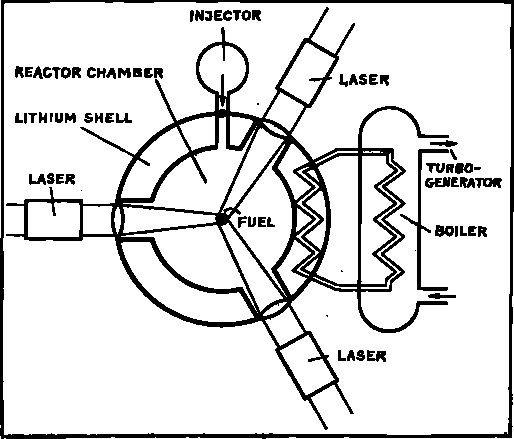
\includegraphics[width=0.9\textwidth]{figures/fig-06-03.pdf}
\caption{A laser based fusion reactor.}
\label{fig-6.3}
\end{figure}

Those are the underlying ideas of the reactor sketched in \figr{fig-6.3}. A solid (frozen) pellet consisting of hydro­gen isotopes falls inside a vessel that has been evacuated to a deep vacuum. When the pellet passes through the centre of the vessel, powerful lasers are switched on that transform the solid into a state of plasma. For the reactor to start up, the energy liberated in the time interval between the start and finish of the reaction must be sufficient to maintain the temperature required to con­tinue the reaction. Calculations show that the plasma must have a density from \num{d3} to \num{d4} times that of the solid, or about \num{d26} particles to every cubic centimetre. A laser is capable of producing the needed compression. 

In principle, it is possible to obtain the requisite tem­perature and density. Then what happens? The fusion energy of the nuclei is conveyed to the neutrons that are released in the reaction. These neutrons fall on the lithium shell of the vessel. The lithium, via a heat exchanger, transfers the energy to a turbogenerator. Part of the neutrons react with the lithium and produce tritium, which is needed as fuel.

The principle is simple but the end is still a long way off, and it is quite possible that fresh and unexpected obstacles will crop up. It is very hard to foresee the requirements of such a reactor when power generation ac­tually begins. Research workers are convinced that pro­ducing such high power outputs in small volumes of substance will reveal entirely new phenomena.


\section{Solar Energy}

The conversion of solar energy to electricity by means of photocells has been known for a long time, but only recently has the idea occurred that this phenomenon could be used as the basis for an electric power plant. The suggestion might appear at first glance to be rather wild. Figure it this way: to make a power plant of 1000 mega­ watts, you would have to cover an area of $6\times6$ square kilometres with \emph{solar cells} (these are special photocells for the conversion of solar energy into electricity). And the calculations are for the sun-drenched Sahara desert. What would you say of a plant like that for the middle of Europe? Here there are not so many sunny days and the area would have to be doubled at the very least. Science fiction, pure and simple, says the reader. Just imagine what a power plant like that would cost to build!

True enough. But compare that with the advantages of such a mode of power generation. We do not use up any material of the earth, we do not pollute the environment with any kind of waste. Aren't those two factors strong enough inducements to get down to a serious study of ways of building cheaper solar cells, optimal arrange­ments of the cells, and the focussing of solar radiation? Many scientists (and I am one of them) are convinced not only that the problem deserves our closest study but hope that precisely this path will lead to electric power plants of the future. In a few years that might very well be problem No. 1.
\begin{figure}[!ht]
\centering
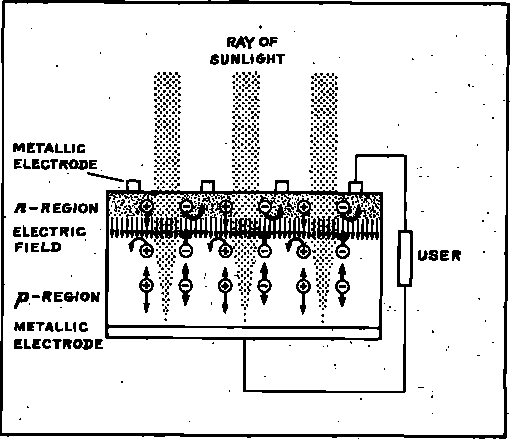
\includegraphics[width=0.8\textwidth]{figures/fig-06-04.pdf}
\caption{A solar cell at work.}
\label{fig-6.4}
\end{figure}

Is not this optimism rather premature? What is the situation today in this field? First of all, what kind of solar cells does industry offer at the present time? 

\figr{fig-6.4} is a diagrammatic sketch of how solar energy is converted into electricity. The cell consists of a semiconductor $p\!-\!n$ layer squeezed between metallic elec­trodes. The sun's rays create free electrons and holes, which are sent in opposite directions by means of a contact voltage, thus generating a current.

There are three main types of such cells. Homocontact cells in which a $p\!-\!n$ sandwich is created by alloying silicon. A diffusion process is used to make a thin (0.3 mi­ crometre) $n$-layer and a relatively thick (300micrometres) $p$-layer. Heterocontact cells consist of two different semiconductors. An $n$-layer of cadmium sulphide is sprayed onto a metallic backing to a thickness of 20-30 micro­metres; then on this surface, chemical methods are used to create a $p$-layer of cuprous sulphide 0.5 micrometre in thickness. A third type of cell makes use of the contact voltage between gallium arsenide and a metal separated by an extremely thin (20 angstroms!) dielectric film.

For optimal utilization of the energy of the whole solar spectrum, semiconductors with electron binding en­ergies of about 1.5 electron volts are suitable. In prin­ciple, efficiencies of 28\% are attainable in solar cells.

Silicon homocontact cells, which have a number of technical advantages and have been studied in the most detail, have efficiencies from 11\% to 15\%. Silicon solar cells have been in use for more than twenty years. The material here is quartz sand (silicon dioxide) from which pure silicon is obtained. Single crystals are manufactured with thicknesses of about 0.3 millimetre in the shape of circular disks. In recent years, a process has been developed for manufacturing monocrystalline tape. The tech­nology of semiconductor doping (the addition of impu­rities to a material) is well developed and permits establishing a $p$-layer in the silicon disk. In order to reduce the reflection of sunlight from the silicon, the surface is covered with a thin film of titanium oxide. With a light intensity of 100 milliwatts per square centimetre, a disk sets up a voltage of 0.6 volt. The current density of a short circuit is equal to 34 milliamperes per square centimetre. There are variety of ways of collecting the cells into batteries. Silicon monocrystalline disks are now being manufactured with diameters from 5 to 7.5 centimetres. They are fixed between plates of glass and can be combined to form a rather powerful source of electric current.

It is hoped that new technological processes will de­velop cells with a much larger area.

The chief obstacle today in the way of using solar cells for industrial power generation is the high cost of manufacturing high-quality monocrystalline tape.

There is considerable hope of making solar cells out of thin polycrystalline layers. The process itself will be cheap but the efficiency will fall drastically. The search is on for cheap methods of obtaining effective solar cells.

At the same time, researchers are seeking ways of increasing the energy falling on a single cell.

There are power plant designs consisting of 34 thousand mirrors reflecting sunlight and directing the radiation to receivers located at the top of a tower 300 metres high.

\begin{figure}[!ht]
\centering

\includegraphics[width=0.4\textwidth]{figures/fig-06-05.pdf}
\caption{Harnessing the energy from the sun.}
\label{fig-6.5}
\end{figure}

If we employ concentrated solar energy, we have to see that the increase in the temperature of the cell does not greatly affect the overall efficiency. In this respect, gal­lium arsenide cells have certain advantages.

Projects are now being considered of siting solar power plants on the top of high mountains where good conditions of solar illumination are ensured. We also have a detailed design of a power plant to be flown on an artificial earth satellite. Such space-borne power plants can receive the energy of solar radiation without any losses and then in the form of microwaves deliver it to the earth where it can be transformed into electricity. And this is not science fiction. Engineers are seriously considering a satellite-borne power plant 25 by 5 kilometres in size. This area could accommodate \num{14000} million photocells! The plant would weigh \num{100000} tons and would generate the equivalent output of several tens of the largest atomic power plants now operating; that is, of the order of ten thousand megawatts.

Detailed projects have already been worked out and small models are undergoing tests.


\section{Power from the Wind}
The air masses of the earth's atmosphere are in constant motion. Cyclones, storms, the constant trade winds of the tropics, and light breezes are only some of the great diversity of energy manifestations of streams of air. The energy of the wind has for ages been used in sailing boats and to drive windmills. The overall mean annual power developed by all air streams over the entire globe comes to the fantastic figure of 100 000 million kilowatts.

Meteorologists are well informed about wind speeds in different places on the globe and at different alti­tudes above the earth's surface. The wind is a temperamental thing and so all estimates involve a mean velocity of 4 metres per second and a mean altitude of 90 metres, which is a modest figure for a coastal strip.

Apparently, the most suitable sites for utilizing the ``blue'' energy of the wind are coastal areas of seas and oceans. It turns out that if Great Britain took advantage of the wind even in rather calm weather (Britain is the richest in wind among the European countries), it could generate roughly six times that produced by all the elec­tric power plants of the country at present. In Ireland, the energy of the winds exceeds electric consumption of the whole country by a factor of one hundred (true, perhaps it is not that there is so much wind but rather so few power plants).

Some twenty or so years ago wind did not rate very high as a source of future power. But the trends of power engineering have been changing before our very eyes. Commissions are set up one after the other to look into the possibilities of new and less expensive sources of energy. The resources of the earth are now regarded in a different light: humanity has begun to think about what is reasonable and what is not as far as utilization of the natural resources hidden in the earth goes. That is why the power of the wind is now being taken seriously. Taking a sober view of engineering possibilities, we may regard as real­istic the harnessing of a fraction of one percent of the 100 000 million kilowatts of available wind power. Even that is a good deal.

\begin{figure}[!ht]
\centering
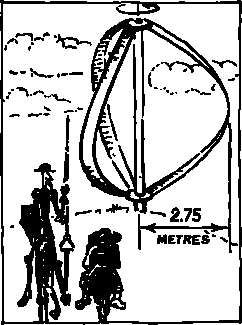
\includegraphics[width=0.5\textwidth]{figures/fig-06-06.pdf}
\caption{A windmill with a vertical rotor.}
\label{fig-6.6}
\end{figure}
Enormous ``windmills'' have already been designed with vanes reaching to 100 metres and more and towers of about that height; windmill vane tips have been calculat­ed to reach speeds of about 500 kilometres per hour. In ordinary weather, a windmill of that class could be expected to have a power capacity of 1 to 3 megawatts. Several thousand such windmills operating in a country with frequent strong winds could supply all the electric­ity needed. In Western Europe, \num{1261.6d12} watt-hours of electric power were generated in 1973. In principle (if one does not skimp on initial outlay) that is but a small part of the energy that can be feasibly extracted from the wind! Gigantic windmills are already under con­struction.


Calculations show that a wind-driven motor has a maximum output when the rotor reduces the wind speed by one third. One should not think that wind-driven units must always imitate windmills. Rotors with a vertical axis of rotation are quite possible. The rotor shown in \figr{fig-6.6} is capable of power outputs of the order of 20 kilowatts. The advantage of such a rotor is its inde­pendence of the direction of the wind; a drawback is that it operates only when there is a strong wind. Rotors of this kind are manufactured with diameters of up to 5.5 metres.

Quite naturally, generators driven by wind must be positioned on a relatively small area, but still at dis­tances apart so that their interaction does not play any role. A power plant with a capacity of 1000 megawatts requires an area of about 5 to 10 square kilometres.


%\begin{figure}[!ht]
%\centering
%
\includegraphics[width=\textwidth]{figures/fig-03-01.pdf}
%\caption{$X$ Rays penetrate muscles and can show the skeleton.}
%\label{fig-3.1}
%\end{figure}

%
%%\newpage
%\begin{center}
%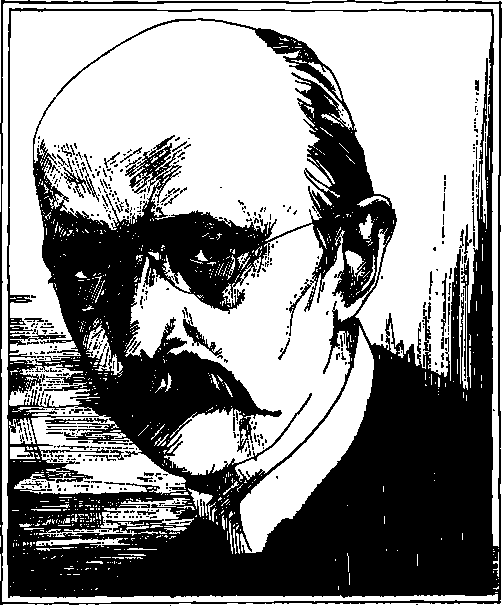
\includegraphics[width=\textwidth]{figures/planck.pdf}
%\end{center}
%{\small \textsf{\hlred{Albert Einstein [1879-1955]}} -- \textsf{\footnotesize the genius who created the theory of relativity and revolutionized all physical thinking. In 1905, Einstein published a treatise devoted to the special theory of relativity. In 1907, he obtained a formula relating energy and the mass of a body. In 1915, Einstein published his general theory of relativity. From this theory there followed new laws of gravita­tion and conclusions concerning the curvature of space.}}



